\section{Public availability, fundamentals and interaction content}\label{sec:supplements}
\subsection{An availability-based comparison}
The existing availability extension dates each completed interaction to day $a$, the first exchange trading day strictly after the last recorded reply, and measures excess returns from close $a$ to close $a+1$. It uses 2017--2024 observations and a separate frozen text calibration. Its manager mean and standard deviation are 0.12749 and 0.21870; the investor anchor is $-0.03150$, the kernel width is 0.32410, $\lambda=0.48115$, and $\gamma=3.04953$. It clips normalized attention above one and omits the historical asymmetric protection. The reference calibration is from 2010--2016; that period is a property of this supplement, not the full-sample historical baseline.

Appendix Table~\ref{tab:public_c2c_regressions} compares ESI with investor tone, manager tone, question volume, substantiveness, both text lengths and Q\&A similarity on 377,721 common observations. The standalone coefficient is 1.48 basis points ($t=4.36$); the full-specification coefficient is 0.58 ($t=0.75$). This horse race does not establish incremental information beyond the complete text set. Existing horizon estimates are also retained. Because sample, calibration and outcome differ from the historical baseline, this comparison does not isolate the effect of changing only the information date.

Appendix Table~\ref{tab:public_c2c_portfolios} holds the candidate pool and 1,786 dates common across all three signals. Domestic CH4 and domestic FF3 cover the actual holding day. FF3 uses CSMAR market P9714 and the circulating-market-capitalization series rather than relabeling the old q5 inputs. ESI's EW CH4 alpha is 4.68 basis points ($t=3.29$); its VW alpha is 3.78 ($t=1.54$). Manager-tone alphas are 4.75 and 6.85. A stable ESI advantage is not established. The supplement retains its exponential annualization convention, explicitly distinguished from the historical arithmetic convention.

\subsection{Actual earnings-announcement dates}\label{sec:fundamental_channel}
The existing fundamental-information test uses CSMAR's report-publication field Annodt. Event day $e$ is the first exchange trading day on or after that date. Signals are averaged over public interaction dates from $e-30$ to $e-3$, requiring at least five signal dates. Missing dates and multiple distinct reports on the same company-event day are excluded. This is an availability-based analysis, not a re-labeling of the historical question-date regression.

In Table~\ref{tab:fundamental_sue}, standalone ESI has an SUE coefficient of 0.0668 ($t=1.07$); with both tones it is 0.1861 ($t=1.07$), using 3,582 observations. The joint ESI coefficient for CH4-adjusted announcement returns is $-22.59$ basis points ($t=-0.27$), using 3,523 observations. Confidence intervals are wide. These tests do not establish additional information about forthcoming earnings; insignificance does not establish the absence of an economic effect.

Earlier significant SUE results used an update-date field. An update date cannot replace the actual publication date when asking which information preceded an announcement. Those tables remain archived and do not support the current fundamental-information claim. Intraday announcement times, analyst earnings forecasts and independently reconstructed accounting vintages remain unavailable.
\begin{table}[H]
\centering
\caption{Public Interaction Signals and Subsequent Earnings}
\label{tab:fundamental_sue}
\footnotesize
\renewcommand{\arraystretch}{1.03}
\setlength{\tabcolsep}{3pt}
\begin{threeparttable}
\begin{tabular*}{\textwidth}{@{\extracolsep{\fill}}l c c c @{}}
\toprule
Predictor & (1) & (2) & (3) \\
\midrule
\multicolumn{4}{@{}l}{\textbf{Panel A: Subsequent SUE}} \\
\midrule
ESI & 0.07 & -- & 0.19 \\
 & (1.07) & -- & (1.07) \\
Investor Tone & -- & 0.15 & 0.07 \\
 & -- & (1.13) & (0.47) \\
Manager Tone & -- & 0.04 & -0.16 \\
 & -- & (0.55) & (-0.81) \\
\midrule
Controls and Firm and Date FE & Yes & Yes & Yes \\
Observations & 3,582 & 3,582 & 3,582 \\
Adjusted $R^2$ & 0.178 & 0.178 & 0.178 \\
\midrule
\multicolumn{4}{@{}l}{\textbf{Panel B: Earnings Announcement Return}} \\
\midrule
ESI & 12.33 & -- & -22.59 \\
 & (0.45) & -- & (-0.27) \\
Investor Tone & -- & -98.97 & -89.17 \\
 & -- & (-1.42) & (-1.11) \\
Manager Tone & -- & 31.38 & 56.14 \\
 & -- & (0.92) & (0.56) \\
\midrule
Controls and Firm and Date FE & Yes & Yes & Yes \\
Observations & 3,523 & 3,523 & 3,523 \\
Adjusted $R^2$ & 0.077 & 0.079 & 0.078 \\
\bottomrule
\end{tabular*}\par
\begin{tablenoteblock}
Day $e$ is the first exchange trading day on or after the CSMAR report publication date, Annodt. Missing publication dates and multiple reports for a firm on the same event day are excluded. Different TestPeriod rows have identical earnings inputs and are counted once per report. Standardized signals are averaged over public interaction dates in $[e-30,e-3]$, requiring five signal dates. Each panel uses a common sample across its three columns. Controls include SUE published by $e-31$, the prior window return, and Size, BM, ROA, Lev, Illiqd, Dturn, and firm age available by $e-31$. Panel A uses the original CSMAR SUE. Panel B sums CH4 abnormal returns over $[e-1,e+1]$ in basis points. Loadings use $[e-252,e-31]$ and at least 120 observations. All regressions include firm and event date effects. Standard errors are clustered by firm and event date. ***, **, and * denote significance at 1\%, 5\%, and 10\%. Intraday announcement times and analyst forecasts are unavailable.
\end{tablenoteblock}
\end{threeparttable}
\end{table}


\subsection{Full-corpus content and question-nature classification}\label{sec:topic_heterogeneity}
We incorporate the completed Qwen3-embedding classification under a supervised, fixed taxonomy of 19 content themes and five question natures motivated by \citet{lee2022shall}. This is content classification rather than unsupervised LDA topic discovery. Questions and replies are classified separately. Production labels remain frozen; this revision does not rerun full-corpus classification.

Technical reconciliation covers 5,836,158 source records and 11,672,316 side-specific predictions. Three question texts are empty. The source contains 234 exact duplicate record combinations, preserved rather than deleted, so record counts are not counts of independent dialogues. Assigned-topic coverage is 54.54\% for questions and 64.49\% for replies. Low-score, generic, context-insufficient and empty cases remain explicit. Coverage is not accuracy: supervision is assistant-generated and independent human semantic evaluation remains pending.

Figure~\ref{fig:topic_distribution} reports content and question nature. Among nonempty questions, the nature shares are 81.56\% answers or explanations, 3.34\% correction of misunderstandings, 1.41\% rumor checks, 3.82\% requests for undisclosed information, and 9.88\% suggestions or other material, subject to rounding. The fourth category retains the figure label ``Inappropriate questions and here denotes requests for undisclosed information; it is not a determination of illegal conduct.
\begin{figure}[H]\centering
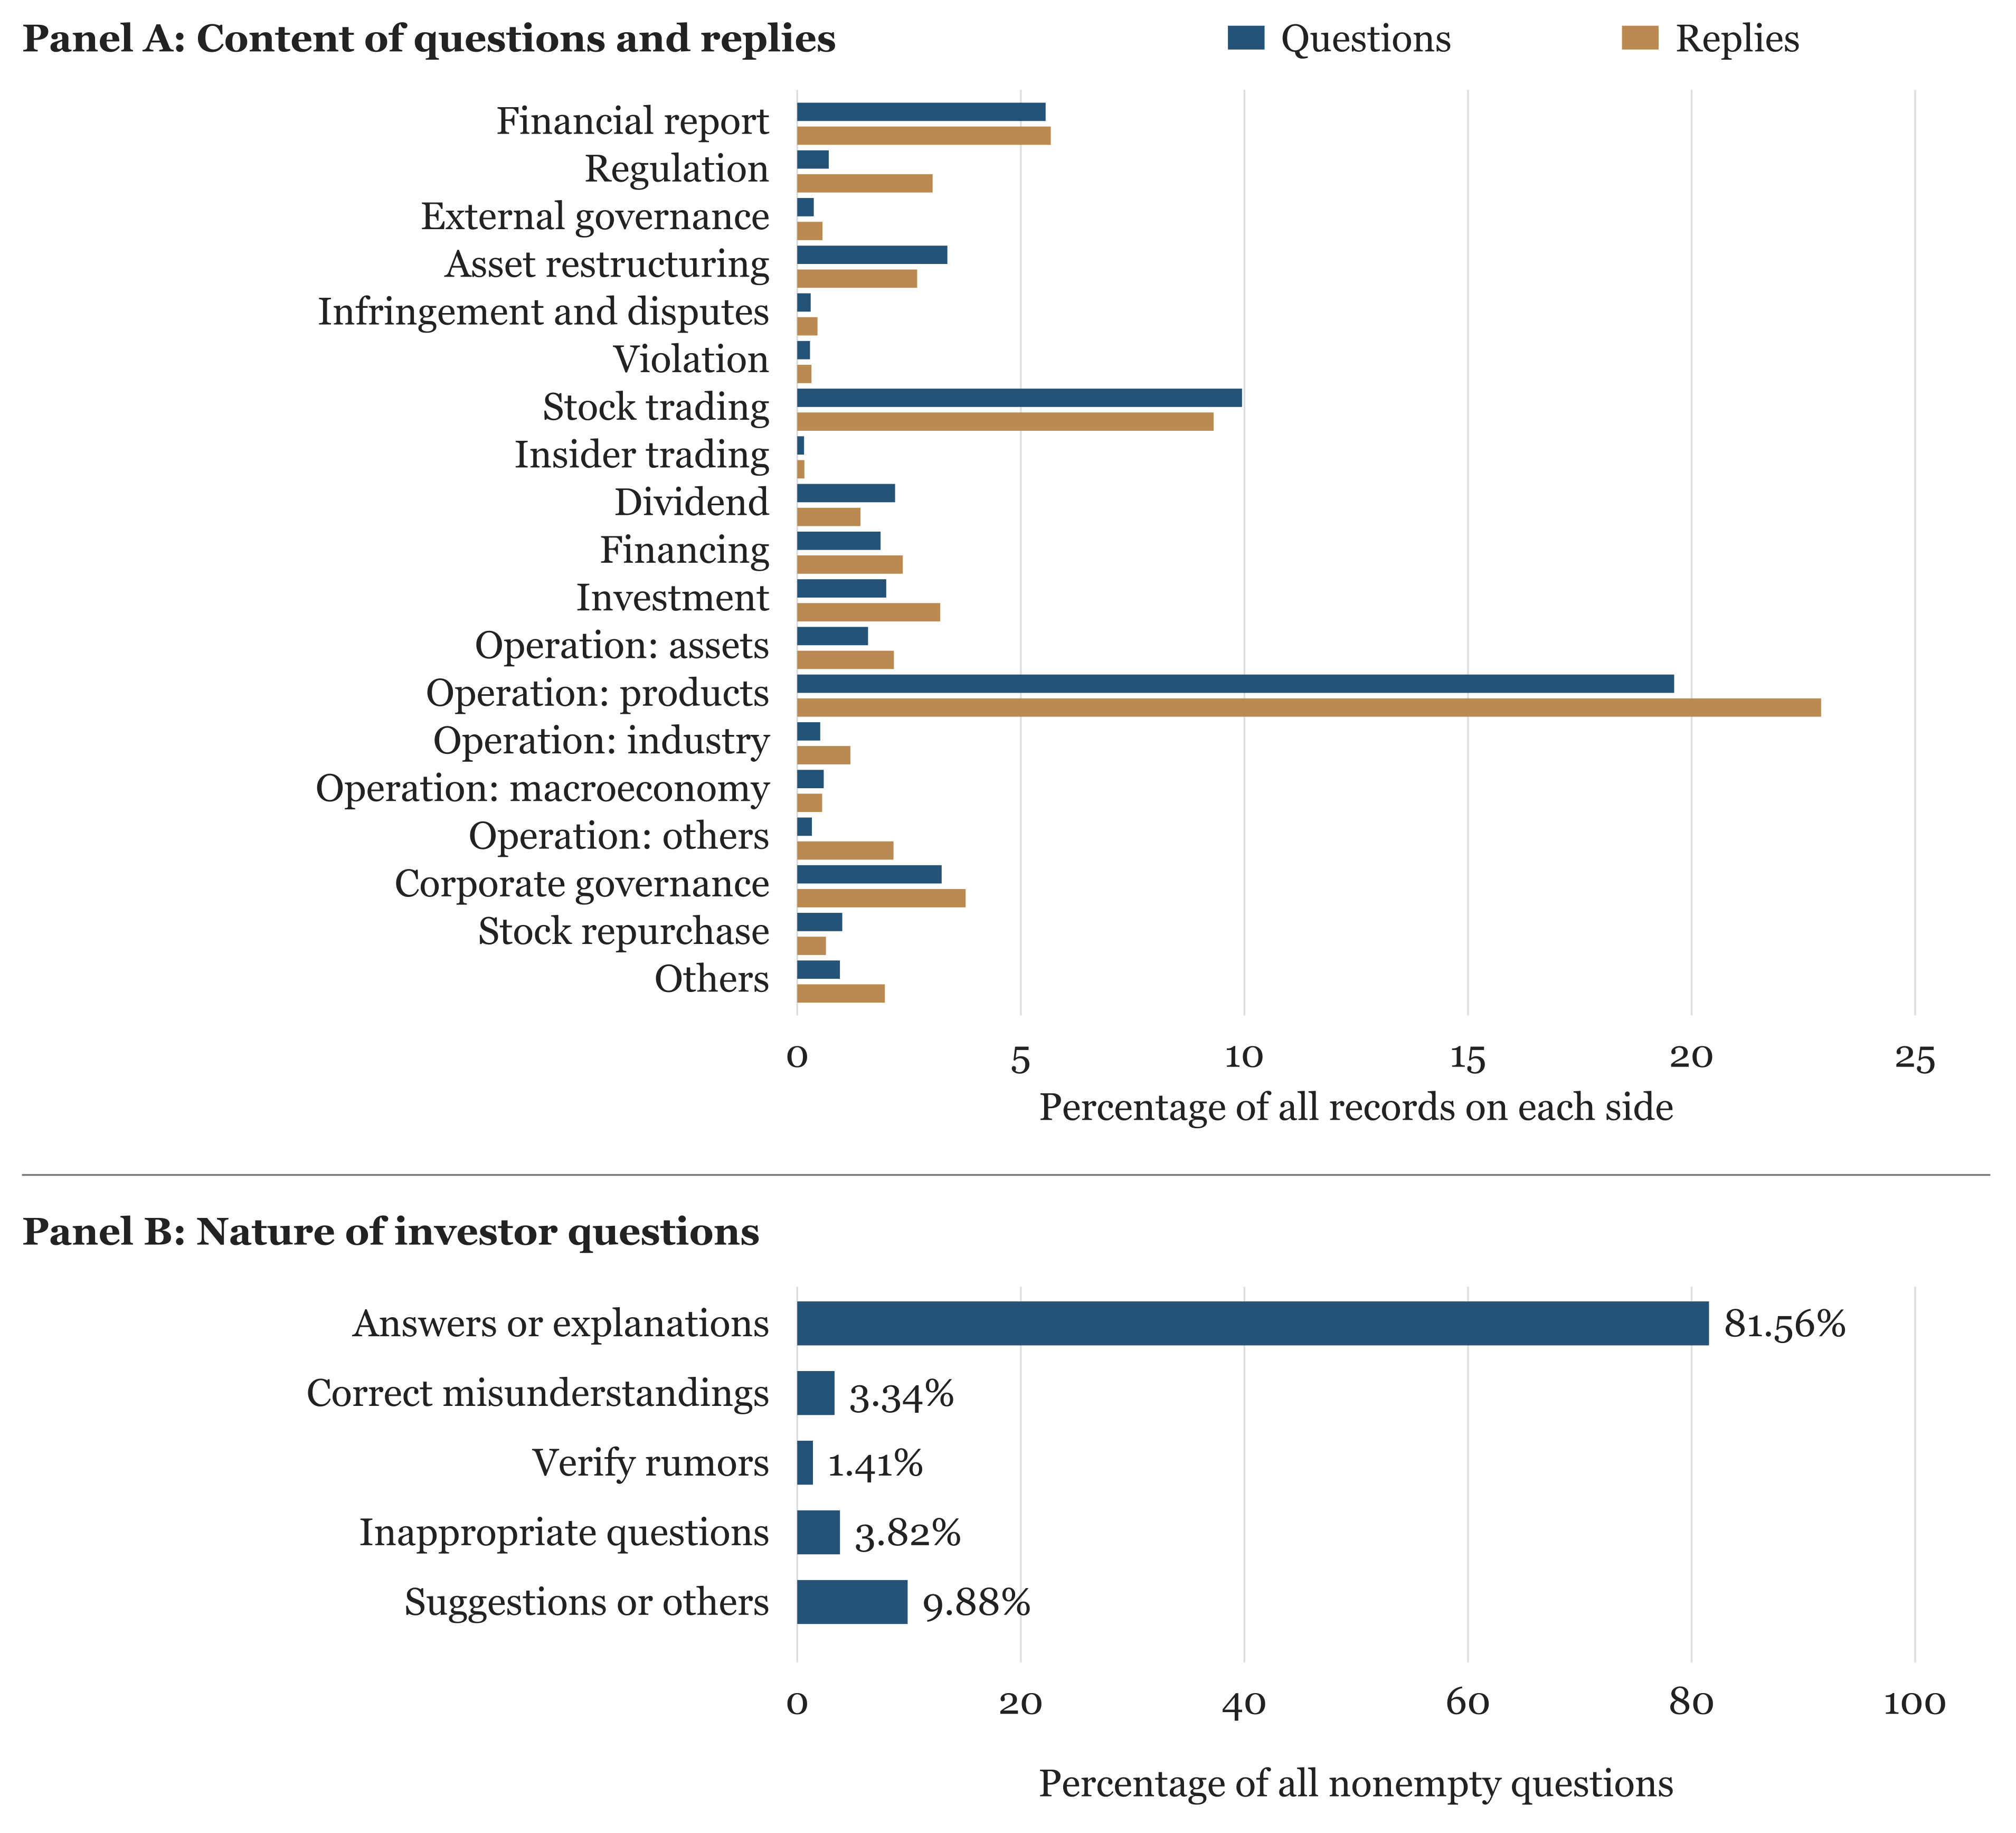
\includegraphics[width=\textwidth]{figures/full_content_and_nature_distribution.png}
\caption{Automated Content and Question Nature Classification}\label{fig:topic_distribution}
\footnotesize Panel A retains the completed question and reply classifications across 19 themes. Its denominator is all source records on each side, including records without an assigned theme, so displayed shares need not sum to 100\%. Panel B uses 5,836,155 nonempty questions. Independent semantic validation remains pending.
\end{figure}

We estimate exploratory C2C slope differences using the dominant question topic at each company-availability date. Let $D_{ik,a}$ indicate category $k$, with unclassified or low-score questions as category 0:
\begin{align}
r^{C2C,e}_{i,a+1}={}&\alpha_i+\delta_a+\beta_0 Z^{ESI}_{i,a}
+\sum_{k=1}^{19}\eta_kD_{ik,a}+\sum_{k=1}^{19}\beta_kZ^{ESI}_{i,a}D_{ik,a}\nonumber\\
&+\boldsymbol c_{i,a}'\boldsymbol\psi+\boldsymbol T_{i,a}'\boldsymbol\rho+\varepsilon_{i,a+1}.\label{eq:topic}
\end{align}
Here $\boldsymbol T$ is omitted in the baseline and contains both tones in the second model. The outcome is next-day C2C excess return, not a CH4 residual. Both models have firm/date effects and two-way clustered errors. Total slopes are $\beta_0$ for category 0 and $\beta_0+\beta_k$ otherwise, in basis points per historical ESI standard deviation.

Table~\ref{tab:full_topic_heterogeneity} retains all 20 categories and both models. Products or business has a baseline slope of 2.02 basis points ($t=3.40$, raw $p=0.000674$, baseline-family BH $p=0.006744$), but 1.12 ($t=1.25$) with both tones. The displayed BH column adjusts the second model's 20 slope tests; its value for this topic is 0.829. Joint slope-equality tests instead test $H_0:\beta_1=\cdots=\beta_{19}=0$, with $p=0.865$ and $0.873$. A significant within-topic slope does not establish a difference from other topics. The analysis remains exploratory.
\begin{table}[H]
\centering
\caption{Exploratory Return Slopes Across Interaction Topics}
\label{tab:full_topic_heterogeneity}
\footnotesize
\renewcommand{\arraystretch}{1.03}
\setlength{\tabcolsep}{3pt}
\begin{threeparttable}
\begin{tabular*}{\textwidth}{@{\extracolsep{\fill}}l c c c c @{}}
\toprule
Dominant Question Content & ESI and Controls & Also Both Tones & BH $p$ & Firm Days \\
\midrule
Unclassified or Low Score & 1.84 (3.44) & 0.97 (1.08) & 0.829 & 180,057 \\
Financial report & 1.04 (0.56) & 0.13 (0.06) & 0.950 & 18,339 \\
Regulation & 5.03 (0.89) & 4.10 (0.72) & 0.829 & 1,125 \\
External governance & -0.15 (-0.01) & -1.16 (-0.07) & 0.950 & 634 \\
Asset restructuring & 3.32 (0.83) & 2.42 (0.60) & 0.829 & 5,507 \\
Infringement, disputes, lawsuit & -8.28 (-0.70) & -9.32 (-0.79) & 0.829 & 738 \\
Violation & -9.77 (-0.62) & -10.83 (-0.69) & 0.829 & 548 \\
Stock trading & 1.22 (1.50) & 0.40 (0.38) & 0.878 & 52,503 \\
Insider trading & -80.80 (-1.10) & -82.10 (-1.11) & 0.829 & 154 \\
Dividend & 1.48 (0.29) & 0.69 (0.13) & 0.950 & 4,169 \\
Financing & -2.47 (-0.59) & -3.44 (-0.80) & 0.829 & 4,590 \\
Investment & 1.84 (0.89) & 0.94 (0.44) & 0.878 & 5,548 \\
Operation operating assets & 2.55 (1.00) & 1.69 (0.64) & 0.829 & 4,681 \\
Operation products or business & 2.02 (3.40) & 1.12 (1.25) & 0.829 & 86,395 \\
Operation industry related & -1.76 (-0.43) & -2.54 (-0.61) & 0.829 & 907 \\
Operation macroeconomic environment & -5.74 (-1.54) & -6.59 (-1.75) & 0.829 & 1,855 \\
Operation others & 3.58 (0.71) & 2.82 (0.55) & 0.829 & 588 \\
Corporate governance & 1.88 (0.45) & 1.05 (0.25) & 0.948 & 5,117 \\
Stock repurchase & 4.07 (0.76) & 3.24 (0.60) & 0.829 & 3,214 \\
Others & -13.17 (-1.36) & -13.81 (-1.42) & 0.829 & 1,057 \\
\midrule
Joint Slope Equality $p$ & 0.865 & 0.873 & -- & -- \\
Adjusted $R^2$ & 0.293 & 0.293 & -- & -- \\
Total Observations & 377,726 & 377,726 & -- & -- \\
\bottomrule
\end{tabular*}\par
\begin{tablenoteblock}
Questions are assigned to 19 fixed content themes and an explicit unclassified category. The dominant category at a firm and availability date is the largest count, including unclassified records. Coefficients are total ESI slopes in basis points per historical standard deviation, not differences from the unclassified reference. Models include category indicators, ESI interactions, baseline controls, and firm and date effects. Errors are clustered by firm and date. The last regression also includes both textual tones. BH probabilities adjust across all topic slopes in that regression. The joint Wald test compares topic slopes rather than counting individually significant estimates. Labels come from assistant supervision and the analysis is exploratory.
\end{tablenoteblock}
\end{threeparttable}
\end{table}

